%%%%%%%%%%%%%%%%%%%%%%%%%%%%%%%%%%%%%%%%%
% baposter Landscape Poster
% LaTeX Template
% Version 1.0 (11/06/13)
%
% baposter Class Created by:
% Brian Amberg (baposter@brian-amberg.de)
%
% This template has been downloaded from:
% http://www.LaTeXTemplates.com
%
% License:
% CC BY-NC-SA 3.0 (http://creativecommons.org/licenses/by-nc-sa/3.0/)
%
%%%%%%%%%%%%%%%%%%%%%%%%%%%%%%%%%%%%%%%%%

%----------------------------------------------------------------------------------------
%	PACKAGES AND OTHER DOCUMENT CONFIGURATIONS
%----------------------------------------------------------------------------------------

\documentclass[landscape,a0paper,fontscale=0.285]{baposter} % Adjust the font scale/size here

\usepackage{graphicx} % Required for including images
\graphicspath{{figures/}} % Directory in which figures are stored

\usepackage{amsmath} % For typesetting math
\usepackage{amssymb} % Adds new symbols to be used in math mode

\usepackage{booktabs} % Top and bottom rules for tables
\usepackage{enumitem} % Used to reduce itemize/enumerate spacing
\usepackage{palatino} % Use the Palatino font
\usepackage[font=small,labelfont=bf]{caption} % Required for specifying captions to tables and figures
\usepackage{url}
\usepackage{vwcol}
\usepackage{tikz}
%\usepackage[hmarginratio=1:1]{geometry}
%\usepgflibrary{qrr.shapes.openrectangle}
\usetikzlibrary{positioning}


\usepackage{multicol} % Required for multiple columns
\setlength{\columnsep}{1.5em} % Slightly increase the space between columns
\setlength{\columnseprule}{0mm} % No horizontal rule between columns

\usepackage{tikz} % Required for flow chart
\usetikzlibrary{shapes,arrows} % Tikz libraries required for the flow chart in the template

\newcommand{\compresslist}{ % Define a command to reduce spacing within itemize/enumerate environments, this is used right after \begin{itemize} or \begin{enumerate}
\setlength{\itemsep}{1pt}
\setlength{\parskip}{0pt}
\setlength{\parsep}{0pt}
}

\definecolor{lightblue}{rgb}{0.145,0.6666,1} % Defines the color used for content box headers

\begin{document}

\begin{poster}
{
headerborder=closed, % Adds a border around the header of content boxes
colspacing=1em, % Column spacing
bgColorOne=white, % Background color for the gradient on the left side of the poster
bgColorTwo=white, % Background color for the gradient on the right side of the poster
borderColor=lightblue, % Border color
headerColorOne=black, % Background color for the header in the content boxes (left side)
headerColorTwo=lightblue, % Background color for the header in the content boxes (right side)
headerFontColor=white, % Text color for the header text in the content boxes
boxColorOne=white, % Background color of the content boxes
textborder=roundedleft, % Format of the border around content boxes, can be: none, bars, coils, triangles, rectangle, rounded, roundedsmall, roundedright or faded
eyecatcher=true, % Set to false for ignoring the left logo in the title and move the title left
headerheight=0.1\textheight, % Height of the header
headershape=roundedright, % Specify the rounded corner in the content box headers, can be: rectangle, small-rounded, roundedright, roundedleft or rounded
headerfont=\Large\bf\textsc, % Large, bold and sans serif font in the headers of content boxes
%textfont={\setlength{\parindent}{1.5em}}, % Uncomment for paragraph indentation
linewidth=2pt % Width of the border lines around content boxes
}
%----------------------------------------------------------------------------------------
%	TITLE SECTION 
%----------------------------------------------------------------------------------------
%
{
\includegraphics[height=4em]{logo.png}} % First university/lab logo on the left
{\bf\textsc{octoDrone: Developing Heterogenous Drone Platforms}\vspace{0.5em}} % Poster title
{\textsc{\{ Alex Henson, Ben De Ivey, Jon Gibson, and William Seymour \} \hspace{12pt} Computer Science, University of Warwick}} % Author names and institution
{
\includegraphics[height=4em]{logo.png}} % Second university/lab logo on the right

%----------------------------------------------------------------------------------------
%	NETWORKS
%----------------------------------------------------------------------------------------

\headerbox{Drone Networks}{name=objectives,column=0,row=0}{

Drones present a powerful way of extending traditional sensor networks, and are currently available at low cost for recreational and commercial use. By allowing for sampling of the environment at any point in 3D space, quadcopters can be more efficient and reduce costs compared to existing systems.

\begin{center}
\includegraphics[scale=0.125]{figures/nevada}

\tiny{A Parrot AR 2.0 quadcopter over the Nevada desert [1]}
\end{center}

Current interesting uses for drone networks being researched include Disaster recovery after earthquakes and flooding, as well as the monitoring of active volcanoes. Most drone networks are heterogeneous: they feature many different models of drones from different vendors, posing a challenge when it comes to creating programs.
}

%----------------------------------------------------------------------------------------
%	SIMULATION
%----------------------------------------------------------------------------------------

\headerbox{Simulation}{name=introduction,column=1,row=0}{
We designed our simulator, octoDrone, to be accessible, extensible, and lightweight. By simulating solutions for drone networks, one can test designs at scale (in order to ensure correctness). This approach also allows for defects to be discovered before deployment to hundreds or thousands of drones.
\newline

Accessibility was achieved by exposing a limited set of API commands which still allowed for the creation of powerful programs. More complicated actions, like routing messages between drones, are handled by separate modules to promote simplicity whilst still allowing for low level control.

\begin{minipage}{0.4\linewidth}
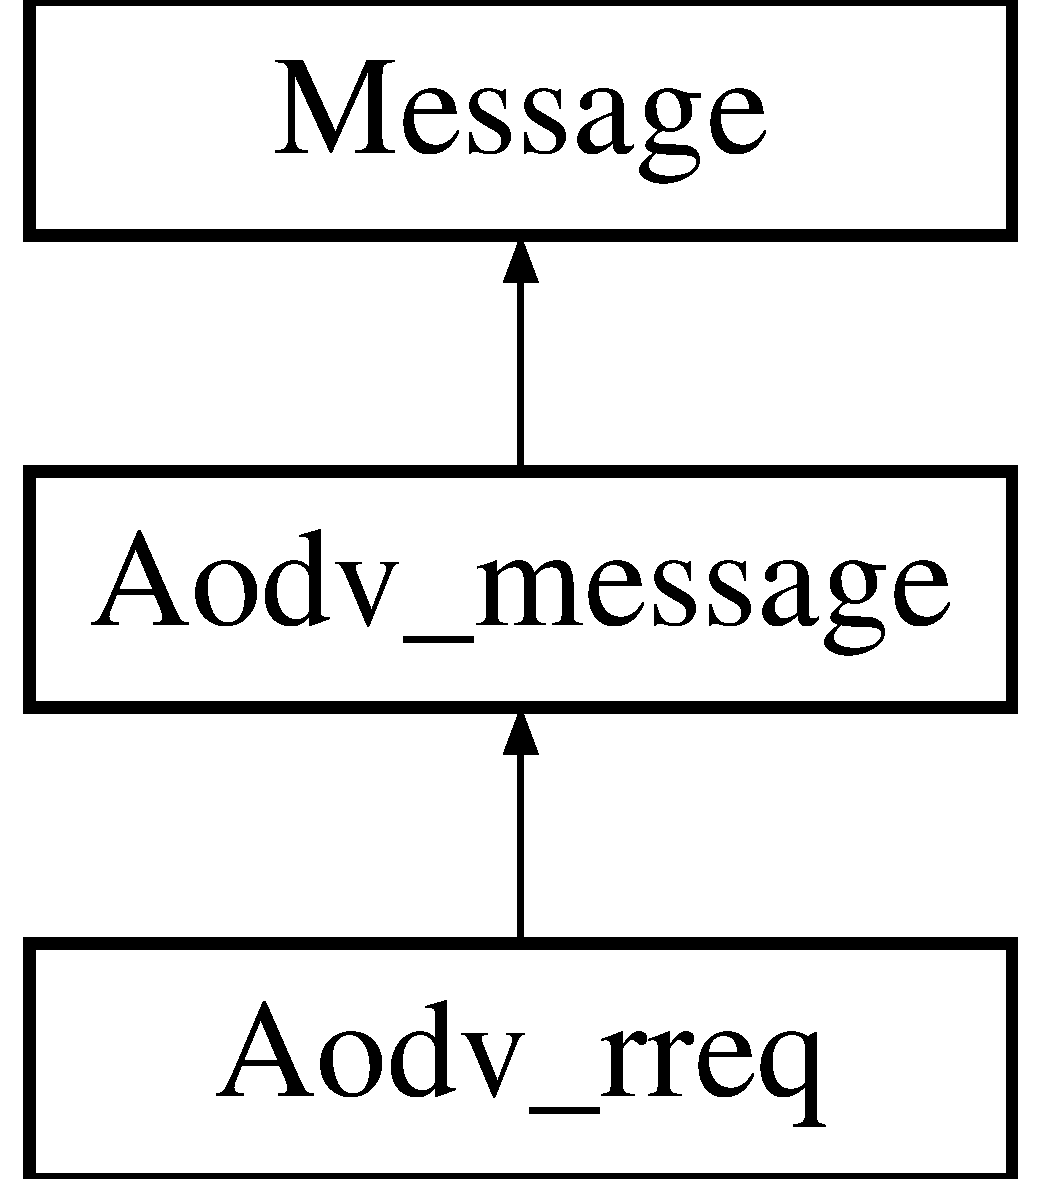
\includegraphics[scale=0.15]{rreq}
\end{minipage}
\begin{minipage}{0.6\linewidth}
In this way, developers can extend existing classes to create their own application specific instances. The AODV RREQ class is a good example of this, extending the AODV message class which itself inherits from a basic message class.
\end{minipage}
\newline

Each drone has separate threads representing its control and communication code. On top of this, the simulation and environment and visualisation layer have additional threads.

\begin{center}
\begin{tikzpicture}[remember picture,
  simulator engine/.style={fill=black!10,rounded corners,inner sep=15pt,inner xsep=5pt},
  topology/.style={rounded corners,draw=blue!50,fill=blue!20,thick,inner sep=3pt},
  neuron/.style={fill=blue!10,draw=blue,rounded corners,inner sep=15pt,inner xsep=5pt,minimum width=3.5cm},
  synapse/.style={draw=red!75,fill=red!20,rounded corners,inner sep=5pt},
  empty synapse/.style={draw=blue!10,rounded corners,inner sep=5pt},scale=0.6, every node/.style={transform shape}
  ]
  \node[simulator engine] (simulatorEngine) {
    \begin{tikzpicture}
      \node[topology] (topology1) {
        \begin{tikzpicture}
          \node [neuron] (neuron1-1)  {
              \begin{tikzpicture}
                  \node [synapse,draw=blue] (synapse1-1-0) {Program Thread};
                  \node [synapse,draw=blue,below=0.1cm of synapse1-1-0] (synapse1-1-1) {Comm Mod Thread};
              \end{tikzpicture}
          };
          \node [neuron,draw=blue,right=0.2cm of neuron1-1] (neuron1-2) {
              \begin{tikzpicture}
                  \node [synapse,draw=blue] (synapse1-2-0) {Program Thread};
                  \node [synapse,draw=blue,below=0.1cm of synapse1-2-0] (synapse1-2-1) {Comm Mod Thread};
              \end{tikzpicture}
          };
          \node [neuron,draw=blue,right=0.2cm of neuron1-2] (neuron1-3) {
              \begin{tikzpicture}
                  \node [synapse,draw=blue] (synapse1-3-0) {Program Thread};
                  \node [synapse,draw=blue,below=0.1cm of synapse1-3-0] (synapse1-3-1) {Comm Mod Thread};
              \end{tikzpicture}
          };
          \node [synapse,draw=blue,below=0.2cm of neuron1-2,minimum width=12cm,minimum height=0.5cm] (synapse1-4) {
          };

          \node [black,below] at (neuron1-1.north)  {Drone A};
          \node [black,below] at (neuron1-2.north)  {Drone B};
          \node [black,below] at (neuron1-3.north)  {Base Station};
          \node [black,below] at (synapse1-4.north)	{Visualisation Thread};
        \end{tikzpicture}
      };

    \end{tikzpicture}
    };

    \node [black,below] at (simulatorEngine.north) {Simulation Environment Thread};
\end{tikzpicture}
\end{center}

Communications modules allow for interrupt driven and time driven messaging. Inbound and outbound message queues are used to keep track of messages waiting to be processed, and the actual passing of messages (after processing) is handled by the simulation environment.
}

%----------------------------------------------------------------------------------------
%	DEPLOYMENT
%----------------------------------------------------------------------------------------

\headerbox{Deployment}{name=results,column=2,span=2,row=0}{
\begin{multicols}{2}
This part of the project aimed to enable the running of octoDrone simulations on real hardware. We adapted the simulator so that sharded instances could be run on each quadcopter. This prevented the need to rewrite correct programs for each type of drone.

%\begin{center}
\begin{tikzpicture}[remember picture,
  simulator engine/.style={fill=black!10,rounded corners,inner sep=20pt,inner xsep=5pt},
  topology/.style={rounded corners,draw=blue!50,fill=blue!20,thick,inner sep=3pt},
  neuron/.style={fill=blue!10,draw=blue,rounded corners,inner sep=15pt,inner xsep=5pt,minimum width=3cm},
  synapse/.style={draw=red!75,fill=red!20,rounded corners,inner sep=5pt},
  empty synapse/.style={draw=blue!10,rounded corners,inner sep=5pt},scale=0.55, every node/.style={transform shape}
  ]
  \node[simulator engine] (simulatorEngine) {
    \begin{tikzpicture}
      \node[topology] (topology1) {
        \begin{tikzpicture}
          \node [neuron] (neuron1-1)  {
              \begin{tikzpicture}
                  \node [synapse,draw=blue] (synapse1-1-0) {Program Thread};
                  \node [synapse,draw=blue,below=0.1cm of synapse1-1-0] (synapse1-1-1) {Comm Mod Thread};
                  \node [synapse,draw=blue,below=0.1cm of synapse1-1-1] (synapse1-1-2) {Comm Server Thread};
                  \node [synapse,draw=blue,below=0.1cm of synapse1-1-2] (synapse1-1-3) {Node Server Thread};
              \end{tikzpicture}
          };
          \node [black,below] at (neuron1-1.north)  {Drone A};
        \end{tikzpicture}
      };

    \end{tikzpicture}
    };

    \node [black,below] at (simulatorEngine.north) {Simulation Thread};
\end{tikzpicture}
\begin{tikzpicture}[remember picture,
  simulator engine/.style={fill=black!10,rounded corners,inner sep=20pt,inner xsep=5pt,},
  topology/.style={rounded corners,draw=blue!50,fill=blue!20,thick,inner sep=3pt},
  neuron/.style={fill=blue!10,draw=blue,rounded corners,inner sep=15pt,inner xsep=5pt,minimum width=3cm},
  synapse/.style={draw=red!75,fill=red!20,rounded corners,inner sep=5pt},
  empty synapse/.style={draw=blue!10,rounded corners,inner sep=5pt},scale=0.55, every node/.style={transform shape}
  ]
  \node[simulator engine] (simulatorEngine) {
    \begin{tikzpicture}
      \node[topology] (topology1) {
        \begin{tikzpicture}
          \node [neuron] (neuron1-1)  {
              \begin{tikzpicture}
                  \node [synapse,draw=blue] (synapse1-1-0) {Program Thread};
                  \node [synapse,draw=blue,below=0.1cm of synapse1-1-0] (synapse1-1-1) {Comm Mod Thread};
                  \node [synapse,draw=blue,below=0.1cm of synapse1-1-1] (synapse1-1-2) {Comm Server Thread};
                  \node [synapse,draw=blue,below=0.1cm of synapse1-1-2] (synapse1-1-3) {Node Server Thread};
              \end{tikzpicture}
          };
          \node [black,below] at (neuron1-1.north)  {Drone B};
        \end{tikzpicture}
      };

    \end{tikzpicture}
    };

    \node [black,below] at (simulatorEngine.north) {Simulation Thread};
\end{tikzpicture}
\begin{tikzpicture}[remember picture,
  simulator engine/.style={fill=black!10,rounded corners,inner sep=20pt,inner xsep=5pt},
  topology/.style={rounded corners,draw=blue!50,fill=blue!20,thick,inner sep=3pt},
  neuron/.style={fill=blue!10,draw=blue,rounded corners,inner sep=15pt,inner xsep=5pt,minimum width=3cm},
  synapse/.style={draw=red!75,fill=red!20,rounded corners,inner sep=5pt},
  empty synapse/.style={draw=blue!10,rounded corners,inner sep=5pt},scale=0.55, every node/.style={transform shape}
  ]
  \node[simulator engine] (simulatorEngine) {
    \begin{tikzpicture}
      \node[topology] (topology1) {
        \begin{tikzpicture}
          \node [neuron] (neuron1-1)  {
              \begin{tikzpicture}
                  \node [synapse,draw=blue] (synapse1-1-0) {Program Thread};
                  \node [synapse,draw=blue,below=0.1cm of synapse1-1-0] (synapse1-1-1) {Comm Mod Thread};
                  \node [synapse,draw=blue,below=0.1cm of synapse1-1-1] (synapse1-1-2) {Comm Server Thread};
				  \node [empty synapse,below=0.35cm of synapse1-1-2] (synapse1-1-e) {};
              \end{tikzpicture}
          };
          \node [black,below] at (neuron1-1.north)  {Base Station};
        \end{tikzpicture}
      };

    \end{tikzpicture}
    };

    \node [black,below] at (simulatorEngine.north) {Simulation Thread};
\end{tikzpicture}
%\end{center}

Because the Parrot AR 2.0 drones used in the project could not be programmed directly, each was paired with a Raspberry Pi running octoDrone. These units were connected via Ethernet, and communicated with the drones via WiFi.
\newline

Messages are sent and received by a communication server thread. An additional piece of middleware written in Node JS (The Node server) [3] is required to translate simulator instructions for a drone into commands that the firmware can interpret (called AT commands).
\newline

\begin{minipage}{0.4\linewidth}
These AT commands are sent by the middleware and include a command (land, hover), sequence number, and some number of arguments.
\end{minipage}
\begin{minipage}{0.6\linewidth}
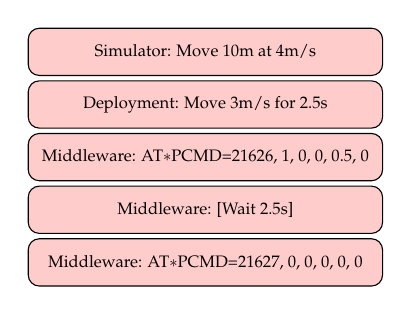
\begin{tikzpicture}[
cell/.style={rectangle, rounded corners, minimum width=7.5cm, minimum height=1cm,text centered, draw=black, fill=red!20, inner sep = 3pt}, arrow/.style={thick,->,>=stealth}, baseline={(current bounding box.east)}, scale=0.6, every node/.style={transform shape}]
	\node (cmd1) [cell] {Simulator: Move 10m at 4m/s};
	\node (cmd2) [cell, below= 0.1cm of cmd1] {Deployment: Move 3m/s for 2.5s};
	\node (cmd3) [cell, below= 0.1cm of cmd2] {Middleware: AT$\ast$PCMD=21626, 1, 0, 0, 0.5, 0};
	\node (cmd4) [cell, below= 0.1cm of cmd3] {Middleware: [Wait 2.5s]};
	\node (cmd5) [cell, below= 0.1cm of cmd4] {Middleware: AT$\ast$PCMD=21627, 0, 0, 0, 0, 0};
\end{tikzpicture}

\tiny{The lifetime of a command, with AT commands as per [4]}
\end{minipage}

\begin{center}
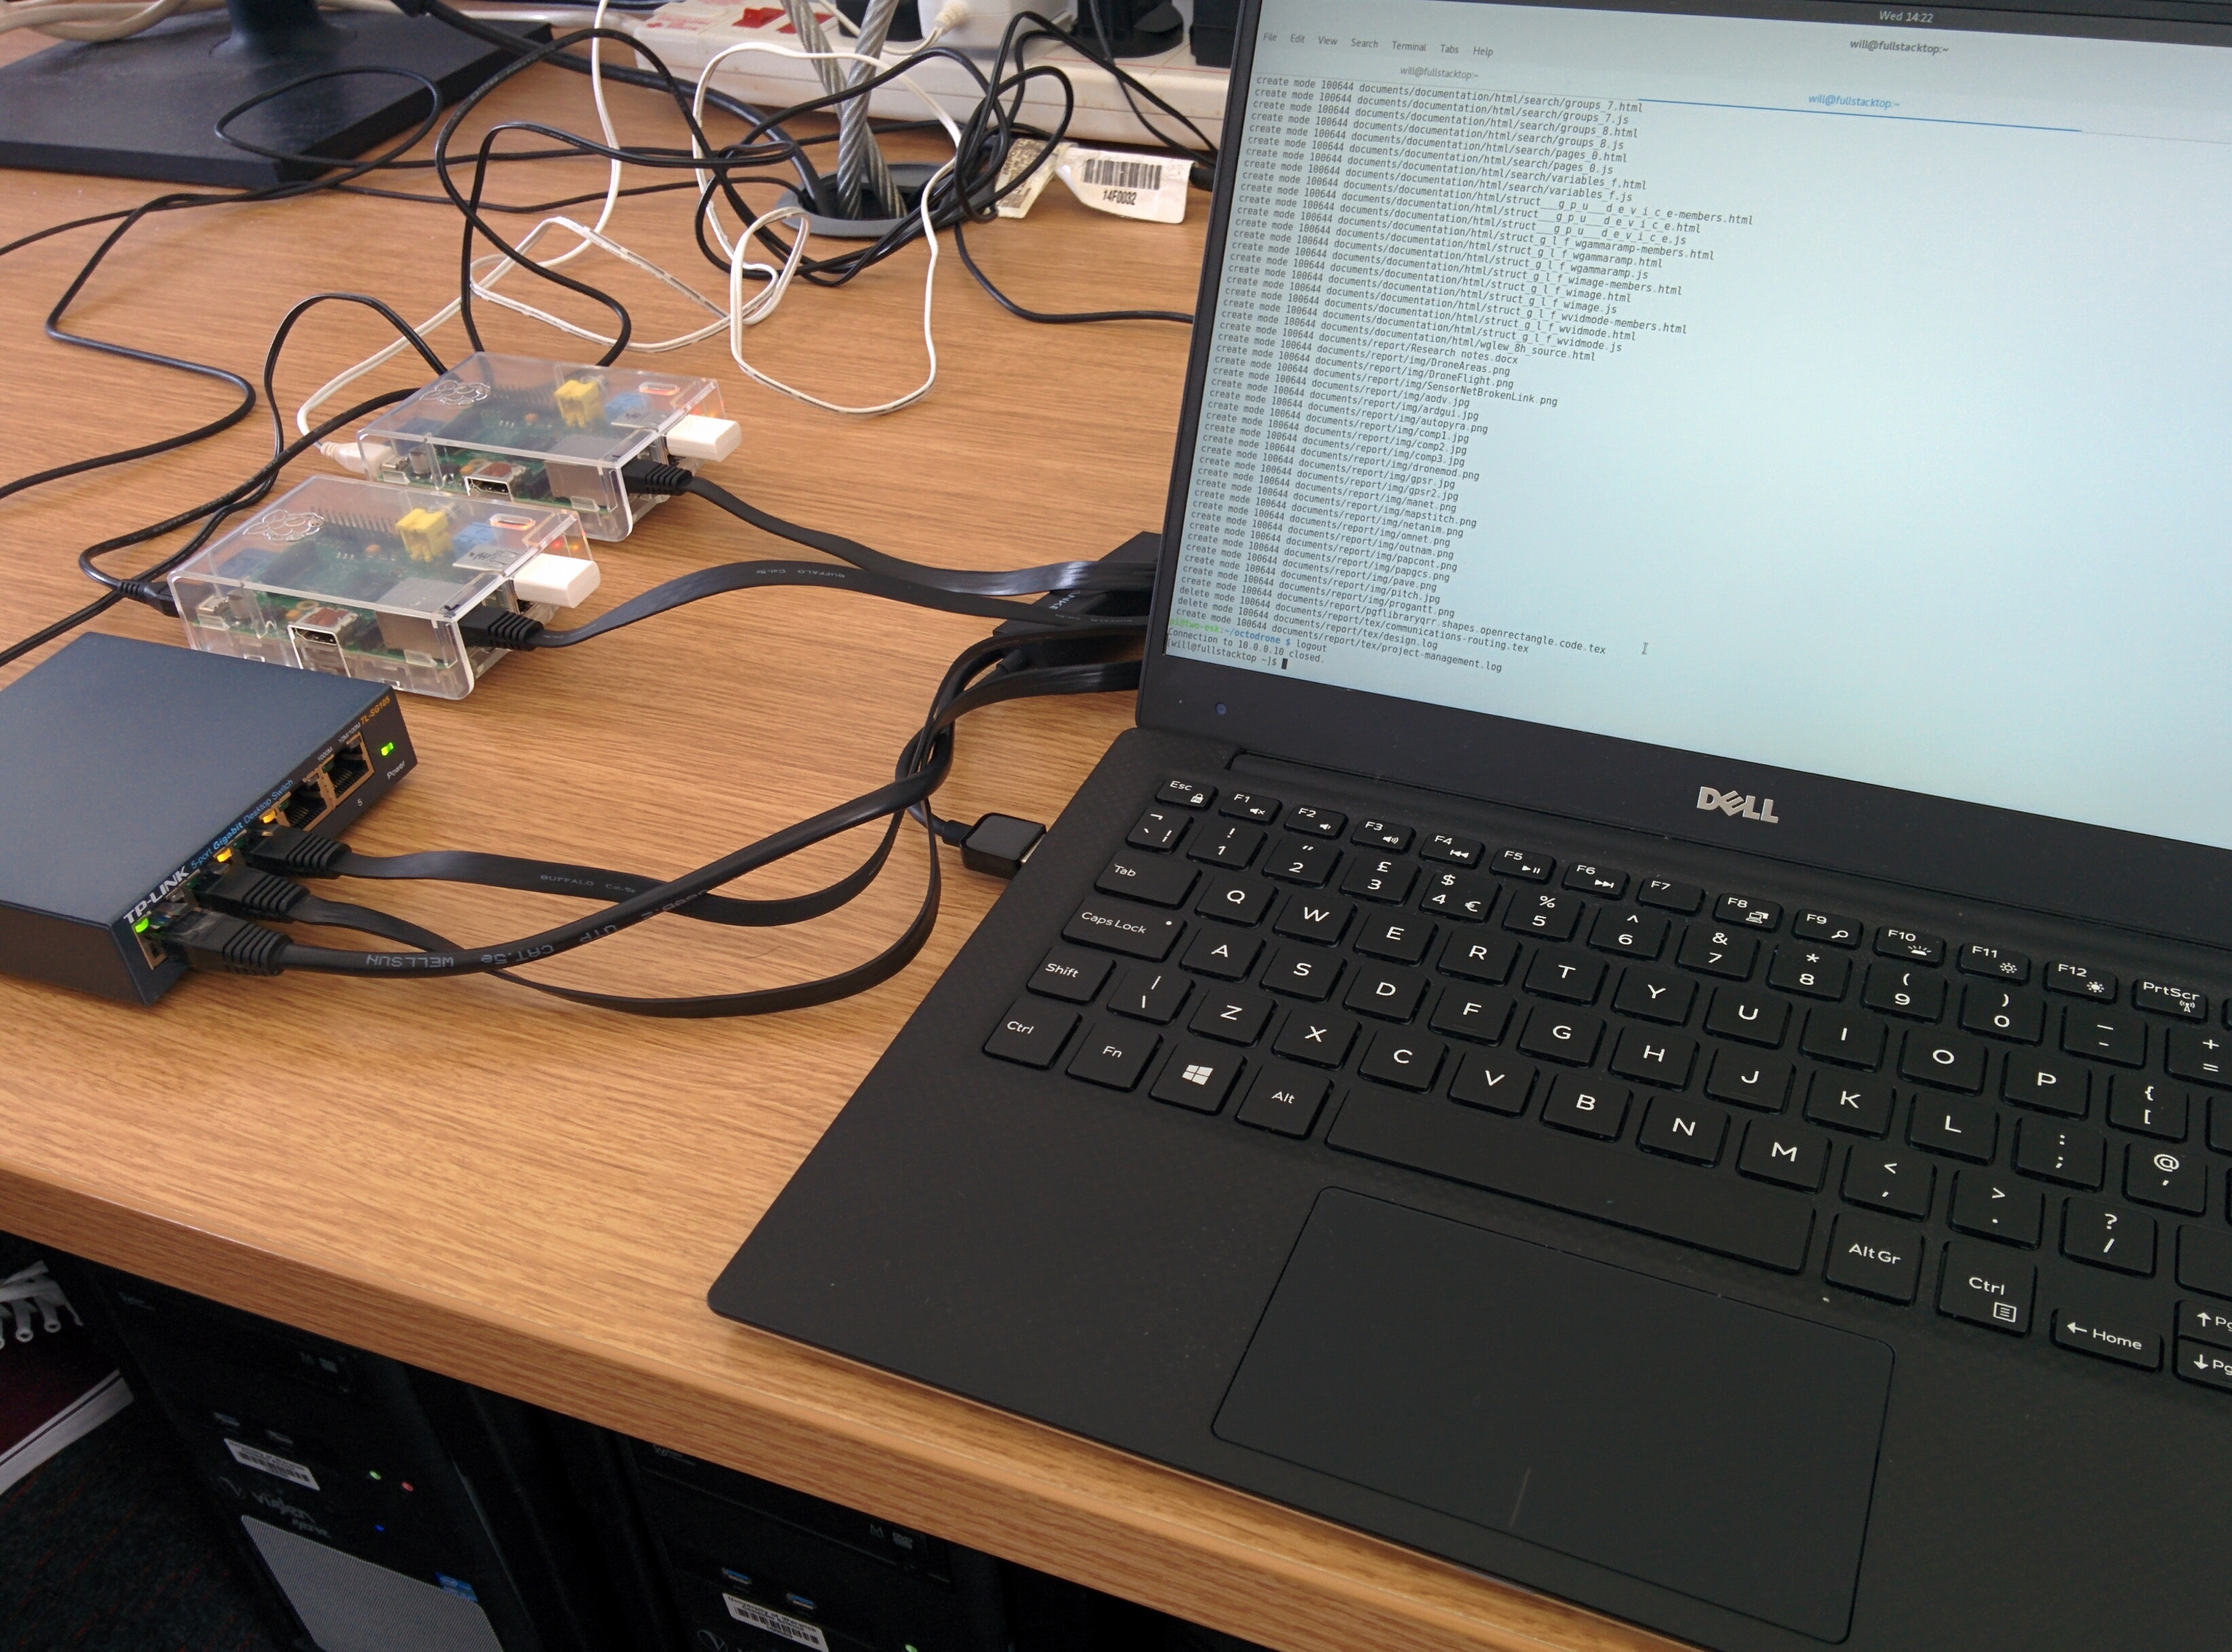
\includegraphics[scale=0.05]{figures/setup}
\end{center}

We were able to successfully demonstrate the deployment capabilities of octoDrone, and show that this approach can be used to make any commercial quadcopter autonomous.

\end{multicols}
}

%----------------------------------------------------------------------------------------
%	REFERENCES
%----------------------------------------------------------------------------------------

\headerbox{References}{name=references,column=0,span=4,above=bottom}{
\begin{multicols}{2}
\scriptsize{ % Reduce the font size in this block
\noindent [1] Parrot SA, 2009. Promotional Materials. [online] Available at $<$\url{http://ardrone2.parrot.com/ardrone-2/specifications/}$>$.


[2] Mottola, L., et al., 2014. Team-level programming of drone sensor networks. 12th ACM Conference on Embedded Network Sensor Systems.

[3] Felix Geisendörfer, 2014. Node JS ar-drone package. [online] Available at $<$\url{https://github.com/felixge/node-ar-drone}$>$

[4] Stephane Piskorski, Nicolas Brulez, Pierre Eline, and Frederic D'Haeyer, 2012. Parrot SA AR Drone Developer Guide.
}
\end{multicols}
}

%----------------------------------------------------------------------------------------
%	USES
%----------------------------------------------------------------------------------------

\headerbox{Use Cases}{name=conclusion,column=2,span=2,row=0,below=results,above=references}{

\begin{multicols}{2}
\section*{Research}
Network simulators form the basis for a large amount of research into sensor networks and IoT devices. By allowing researchers to test their work under real world conditions, more representative results can be obtained, leading to better research.
\newline

Additionally, octoDrone is flexible enough to allow for almost any conceivable feature to be implemented with minimal effort. This modular approach is vital when research requirements are changing rapidly in this evolving field.
\section*{Outreach}
With sensor networks, demonstrating research to students and members of the public can be difficult due to the many layered mechanics involved. Simulation offers a visual means of presenting this information, making it easier to understand.
\newline

Being able to deploy programs to drones opens up opportunities in schools, where hands on time with hardware is at a premium. Being able to see a physical result for their work is a great motivator for students.
\end{multicols}
}

%----------------------------------------------------------------------------------------
%	OBJECTIVES
%----------------------------------------------------------------------------------------

\headerbox{Objectives}{name=method,column=0,below=objectives,bottomaligned=conclusion}{ % This block's bottom aligns with the bottom of the conclusion block

The aim of the project was to create a platform for the simulation and deployment of drone-based sensor networks. We aimed to develop a generic solution to the problem of modelling airborne sensor networks, including those comprised of heterogeneous hardware.
\newline

We aimed to  demonstrate the effectiveness of the simulator by establishing a framework for running simulations on real hardware, without requiring users to change their program code. We hope that this solution will provide a basis for teaching, and research into the way that these networks are used in the future.
}

%----------------------------------------------------------------------------------------

\end{poster}

\end{document}